\chapter{NDVI-MAP FUNCTIONS AND USER GUIDE}
\label{chap:ndvi & it's user guide}

\section{What can app do?}

Application can enable you to envision \gls{ndvi} mean information for any date accessible in the database. It likewise gives the usefulness of sending out the information into \gls{csv} record and messaging it to whosoever you need. It likewise causes you visualize information utilizing diverse levels - Country wise, State wise and District.

\section{A user guide/manual}

A guide is a short reference to some particular aspects of a software product. The examples can be all kinds of ‘How-to’, ‘Installation’ and ‘Getting Started’ guides. Interestingly, user guides can be created both in a form of written documents (e.g. troubleshooting guides with step-by-step explanations) and in the form of different media, such as help video. In this thesis, it has been explained in the form of written document.

\begin{itemize}
    \item \textbf{Downloading the app} \\
    Right now, the app is in process of being submitted to App Store for review. Once it is approved by Apple, you can utilize the "EyesOnCrops" application by downloading it from the Apple Store. 
    
    \begin{itemize}
        \item Open the App Store and type "EyesOnCrops" in search bar.
        \item Download and introduce the "EyesOnCrops" application on your gadget.
        \item Once installed, it will look like Figure~\ref{fig:app_icon_screen} on your device.
        
        \begin{figure}[H]
            \centering
            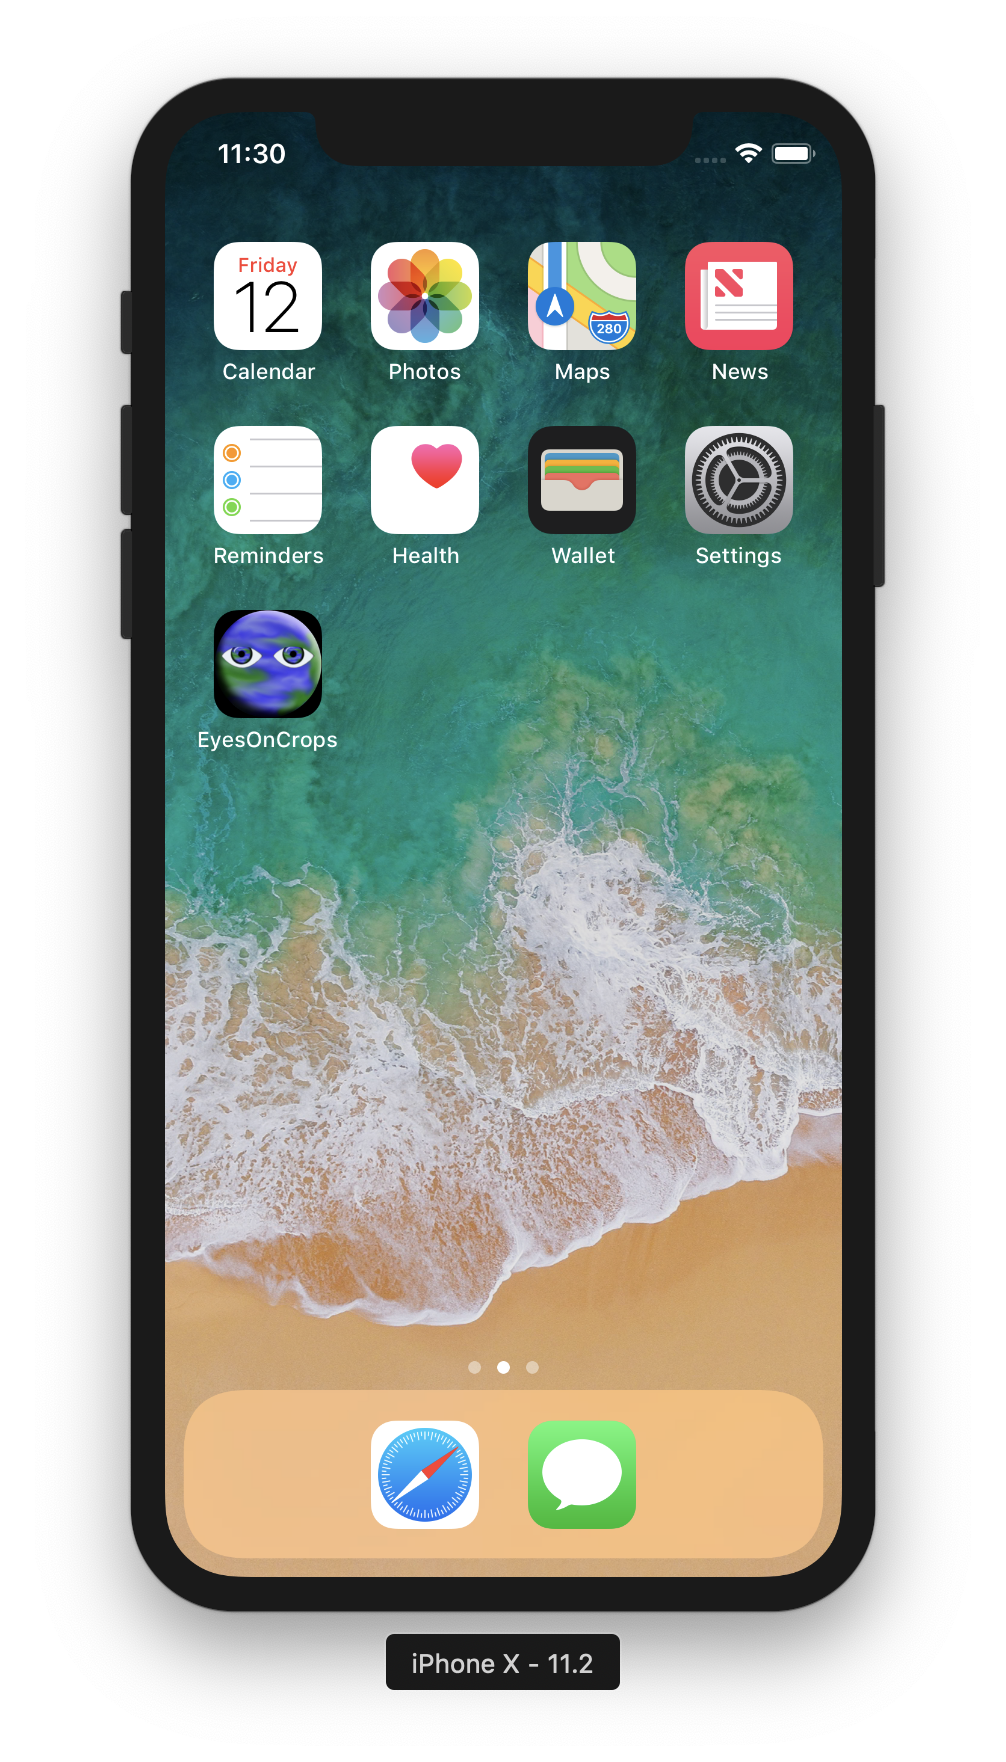
\includegraphics[width=0.50\linewidth]{figures/ch2/app_icon_screen.png}
            \caption{\label{fig:app_icon_screen} iPhone screen after downloading the app}
        \end{figure}
    \end{itemize}
    
    \item \textbf{Getting in the app} \\
    By tapping on app icon on Figure~\ref{fig:app_icon_screen}, it will lake you to landing screen of the app, also known as the main screen. This screen gives you two options, which are (as shown in figure 2.2).
     
        \begin{figure}[H]
            \centering
            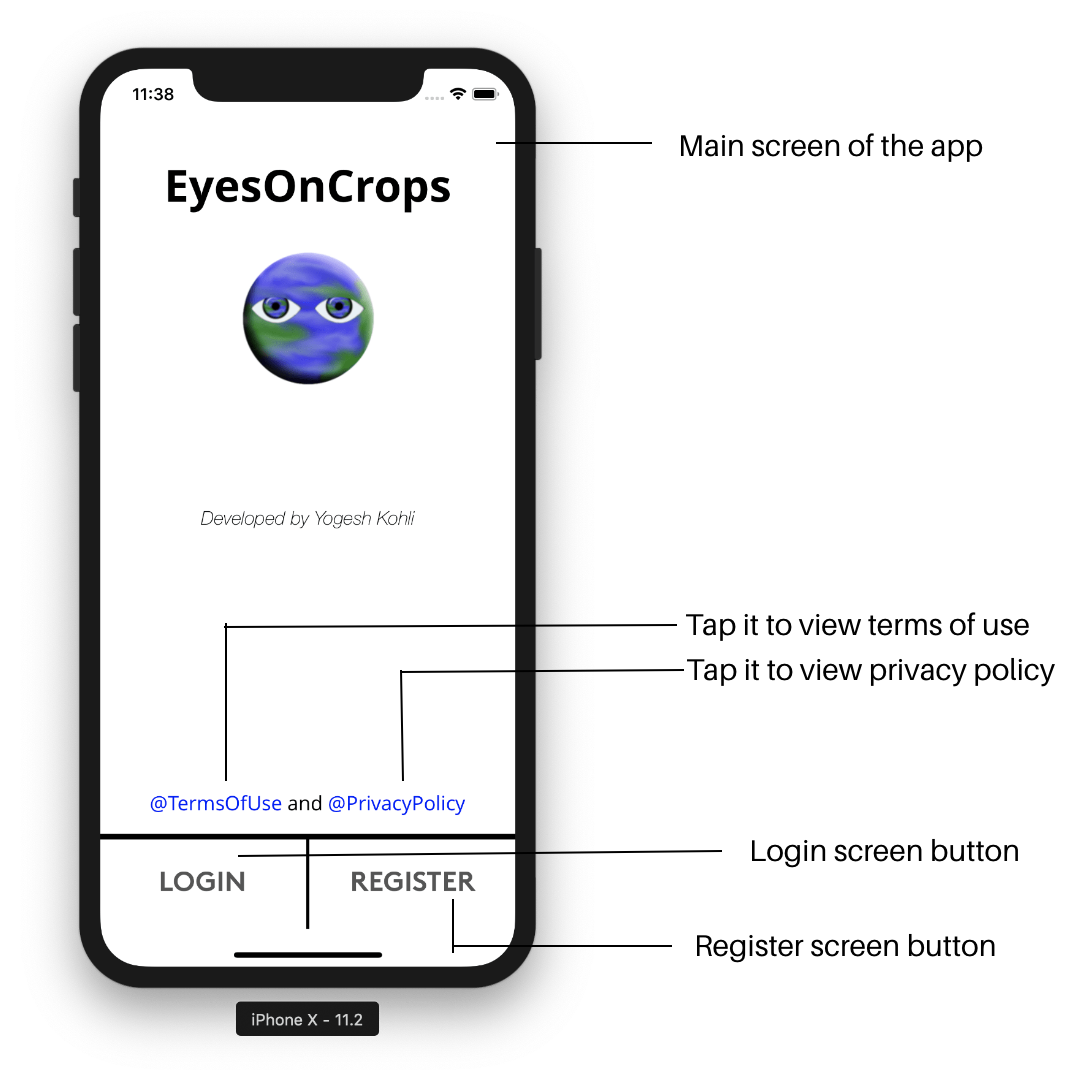
\includegraphics[width=0.50\linewidth]{figures/ch2/main_screen.png}
            \caption{\label{fig:main_screen} Main / Landing screen of the app}
        \end{figure}

    \textbf{1. Register} \\
    \textbf{2. Login} \\
    
    If you select \textbf{Register} in Figure~\ref{fig:main_screen}, it takes you to registration process. Registration process has been divided into 5 steps which are explained below.
    
    
        \begin{figure}[H]
            \centering
            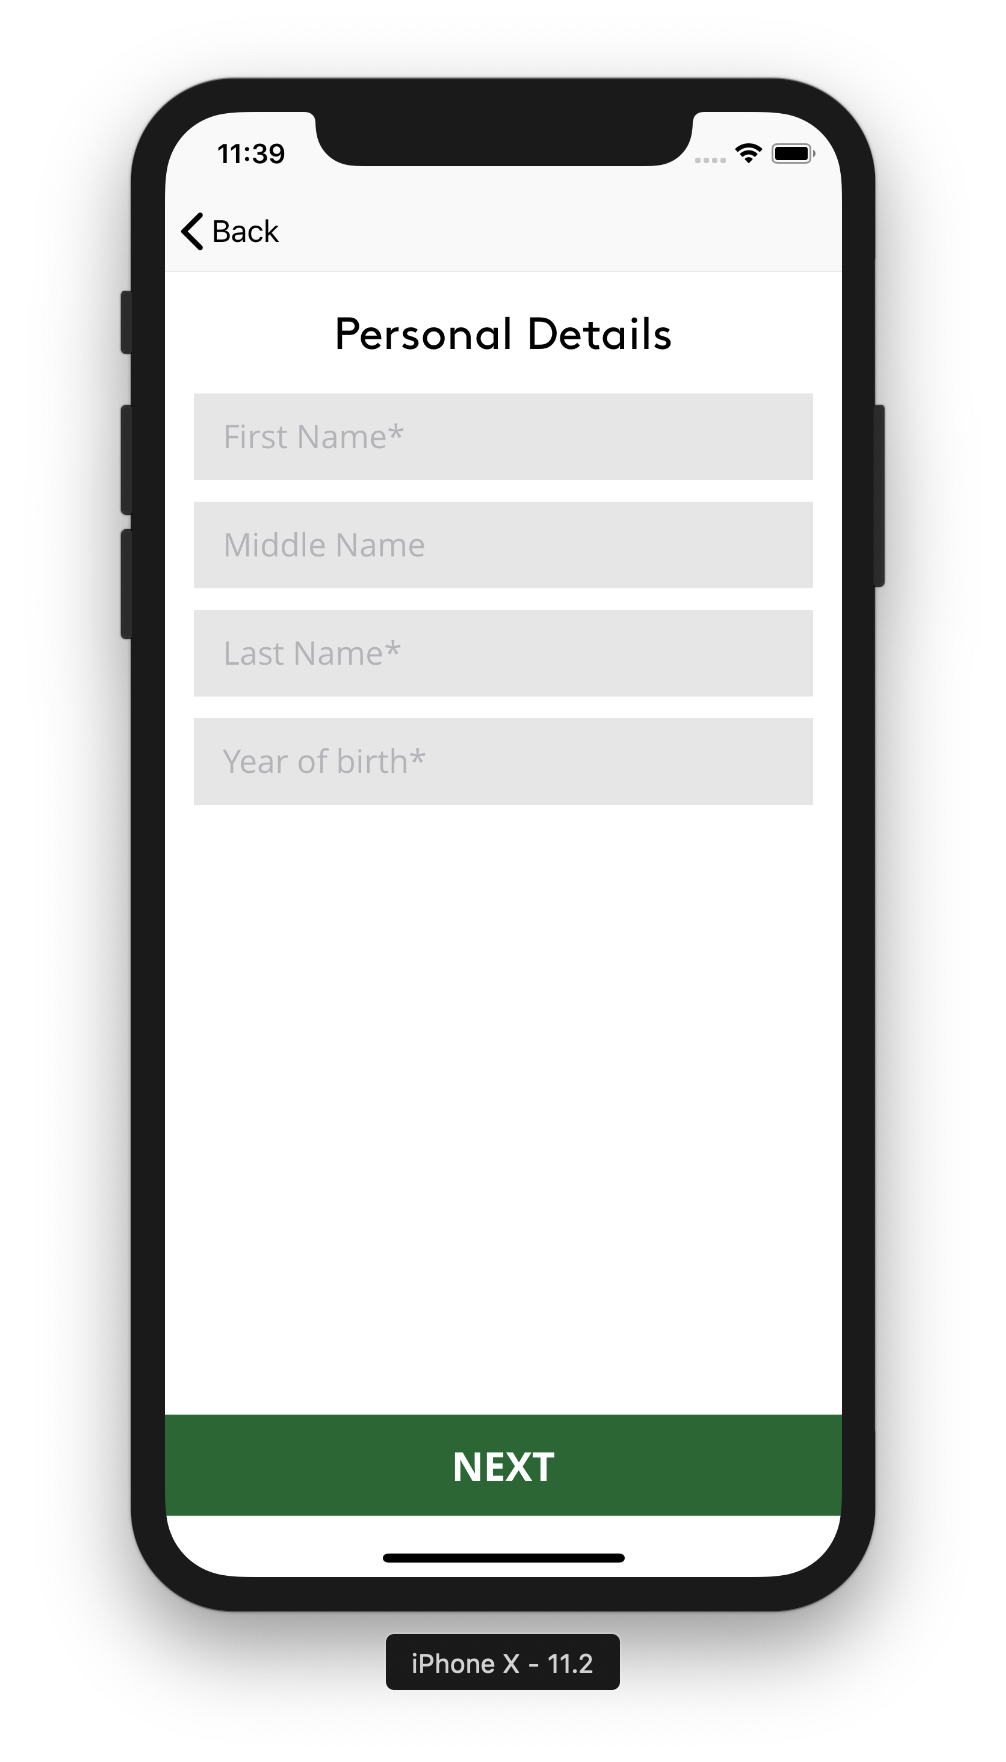
\includegraphics[width=0.50\linewidth]{figures/ch2/register_personal.png}
            \caption{\label{fig:register_personal} Personal details screen - Register process}
        \end{figure}
  
        
        \begin{figure}[H]
            \centering
            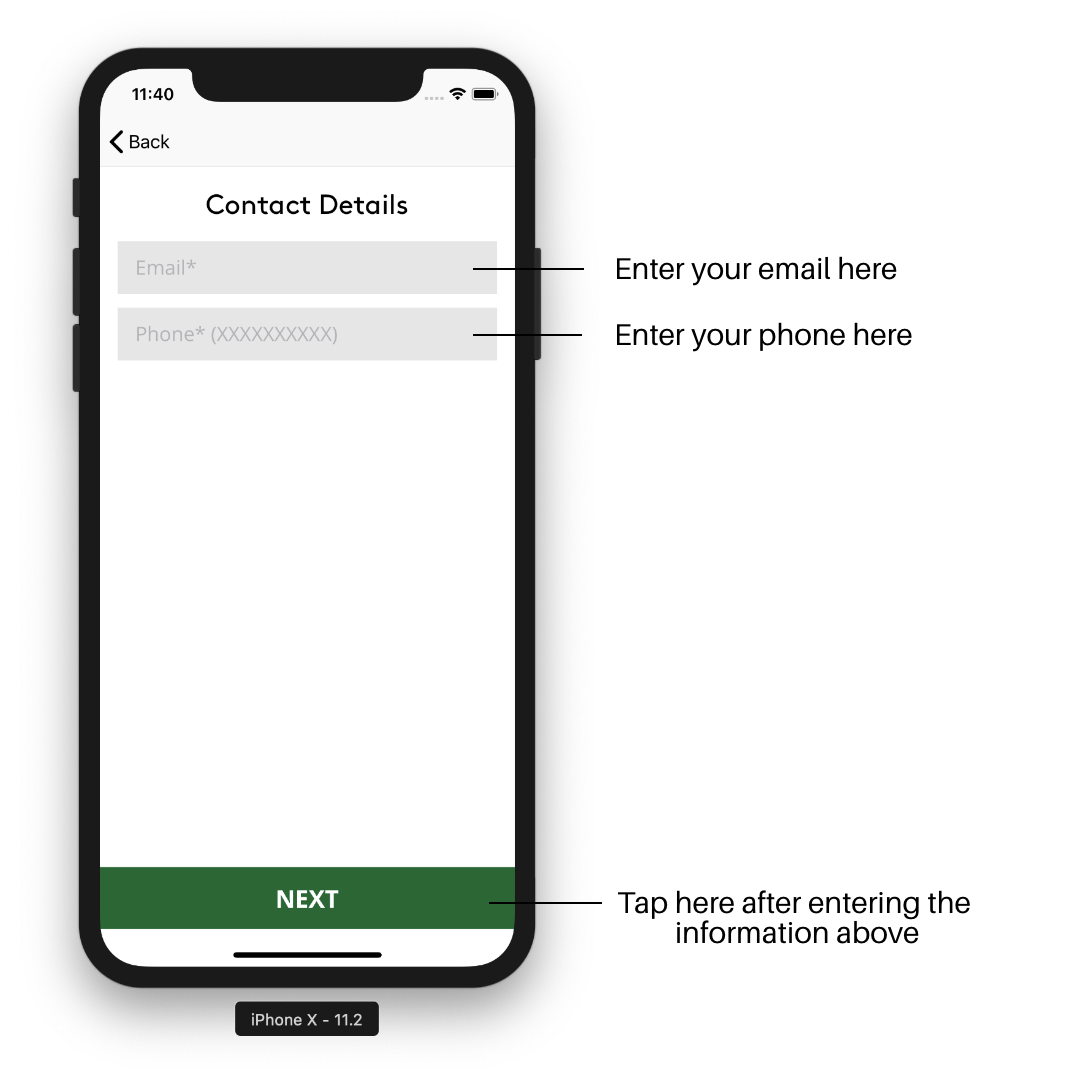
\includegraphics[width=0.50\linewidth]{figures/ch2/register_contact.png}
            \caption{\label{fig:register_contact} Contact details screen - Register process}
        \end{figure}
     
        \begin{figure}[H]
            \centering
            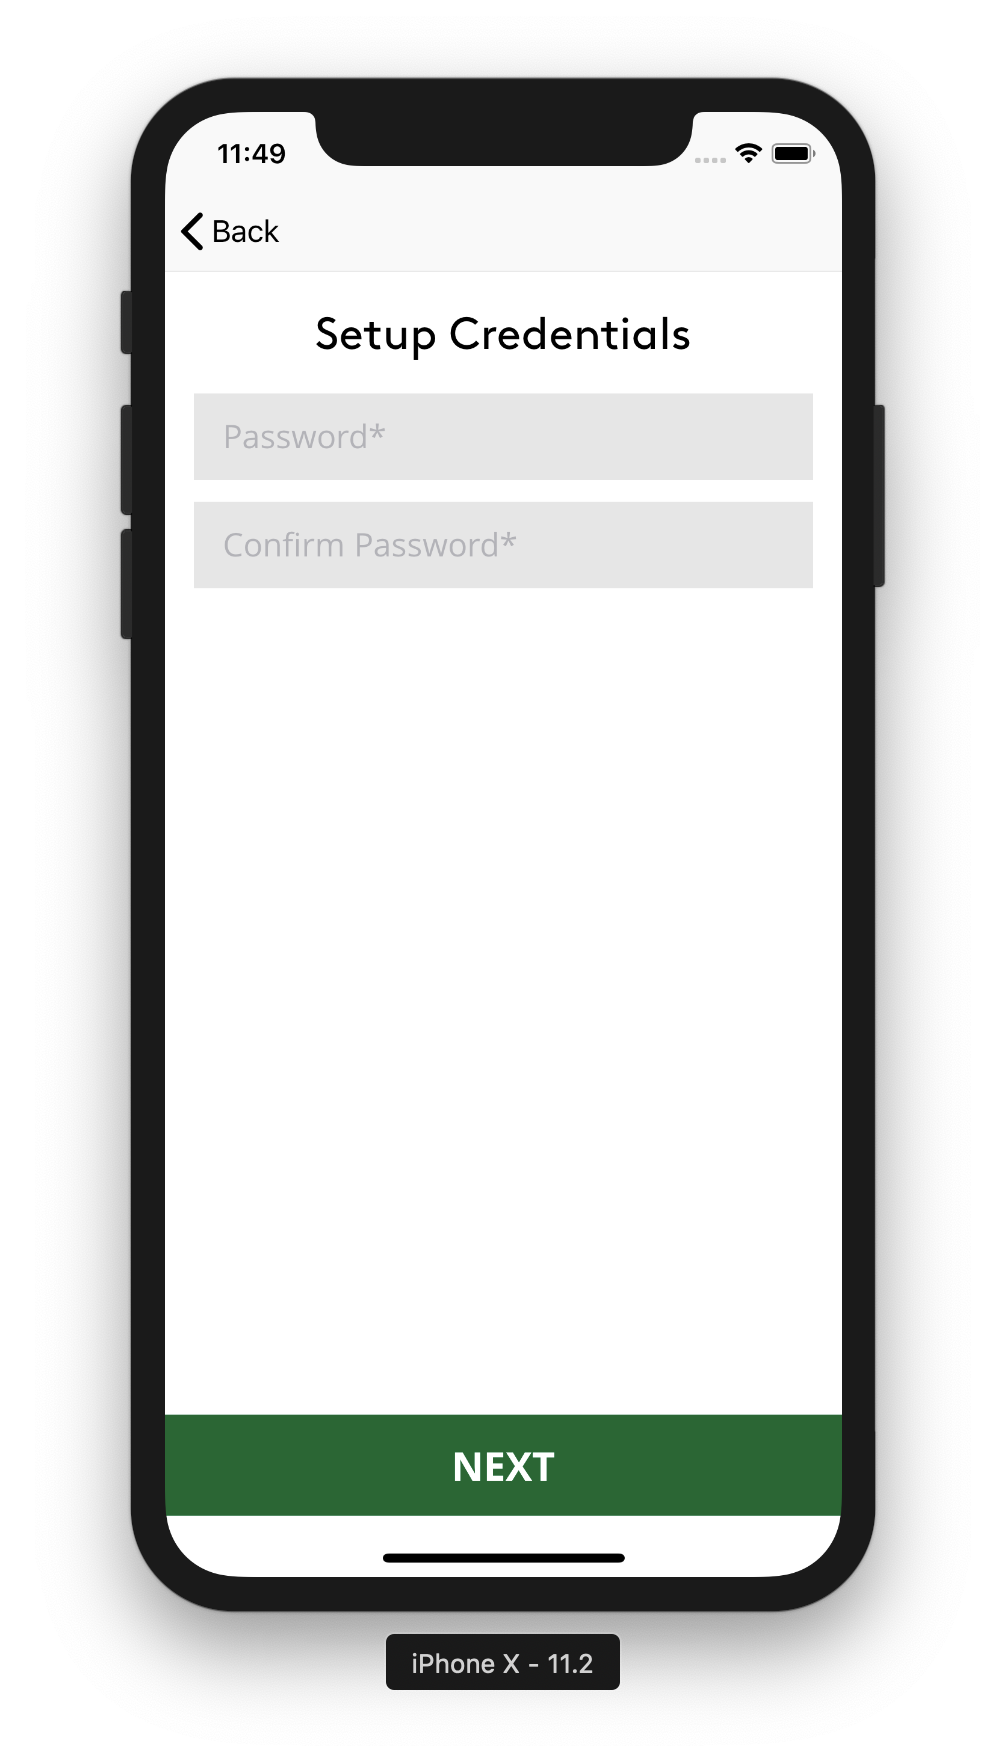
\includegraphics[width=0.50\linewidth]{figures/ch2/credentials_setup.png}
            \caption{\label{fig:credentials_setup} Setup credentials screen - Register process}
        \end{figure}
       
        
        \begin{figure}[H]
            \centering
            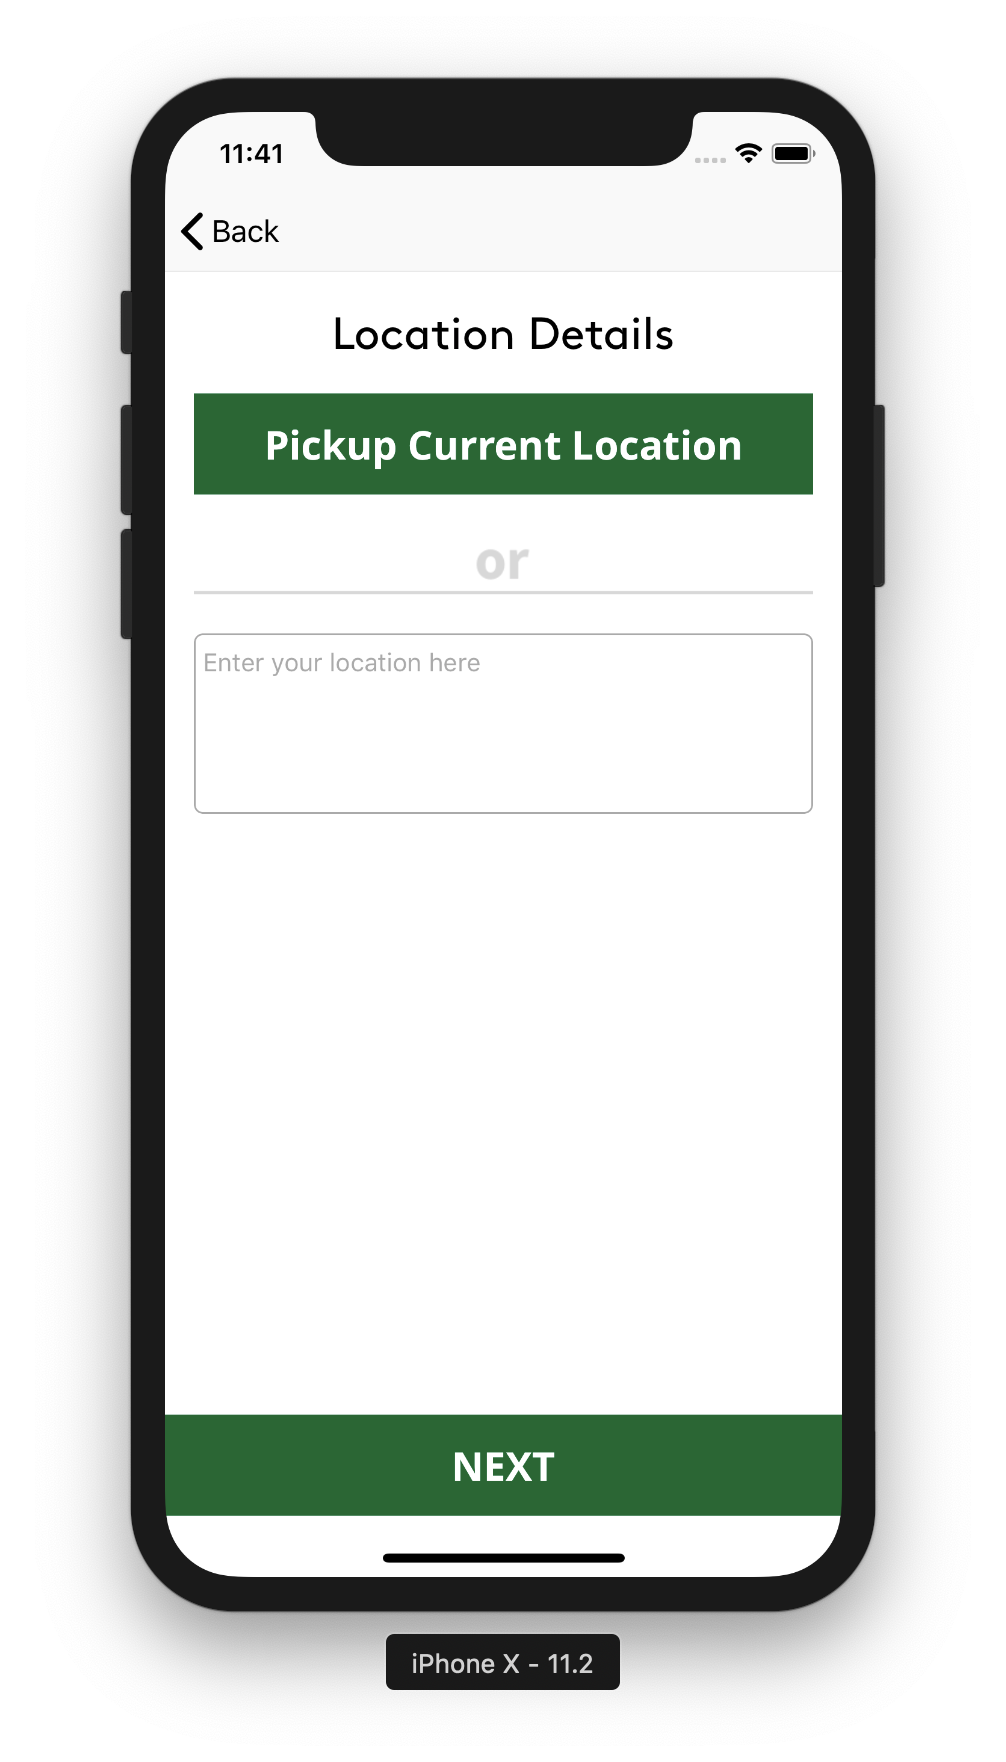
\includegraphics[width=0.50\linewidth]{figures/ch2/register_location.png}
            \caption{\label{fig:register_location} Location details screen - Register process}
        \end{figure}
 
        \begin{figure}[H]
            \centering
            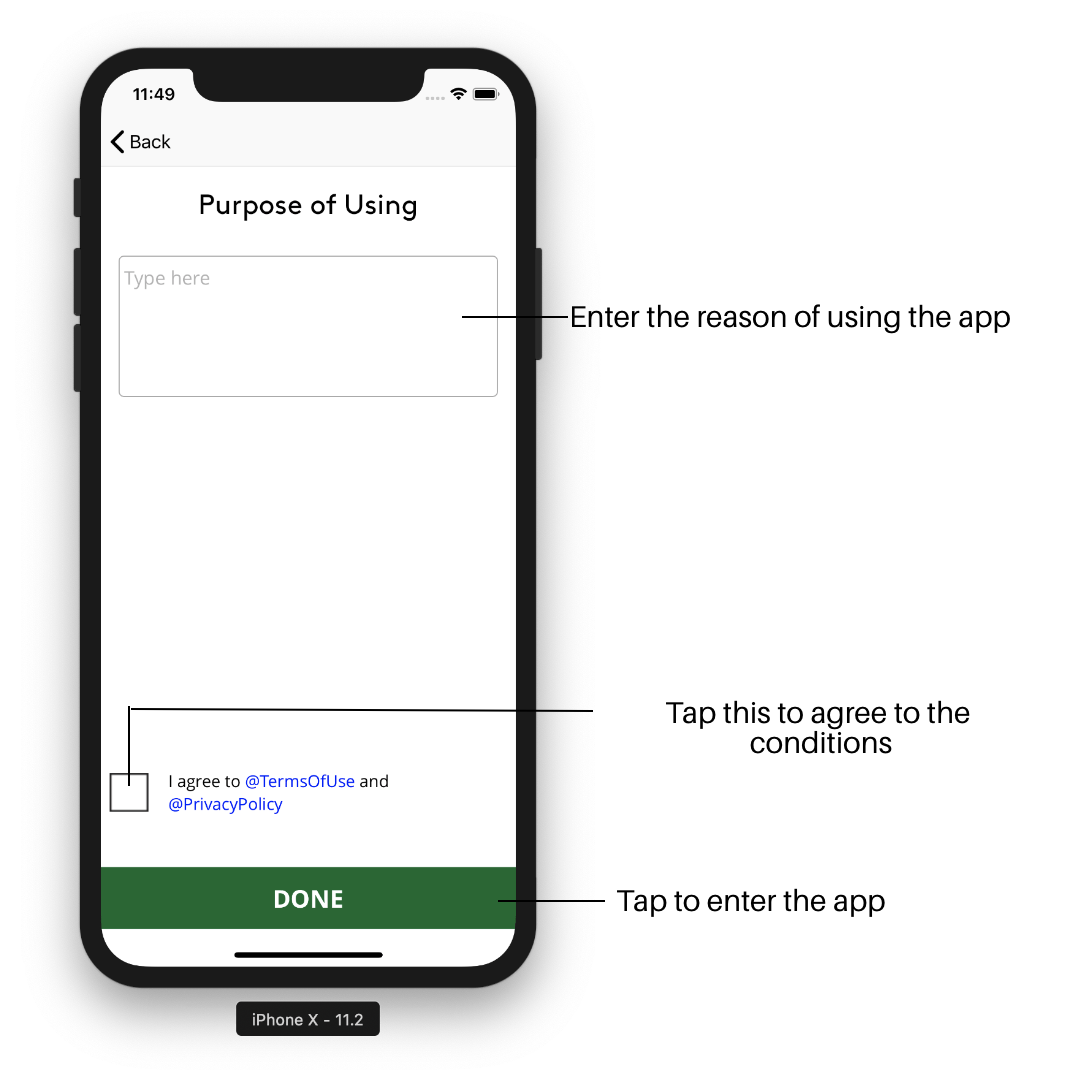
\includegraphics[width=0.50\linewidth]{figures/ch2/purpose_app.png}
            \caption{\label{fig:purpose_app} Purpose of using the app screen - Register process}
        \end{figure}

    
    If you select \textbf{Login} in Figure~\ref{fig:main_screen}, it takes you two that screen which gives you options to enter the app which is shown in Figure~\ref{fig:loginOptions}.
    
    \begin{figure}[H]
            \centering
            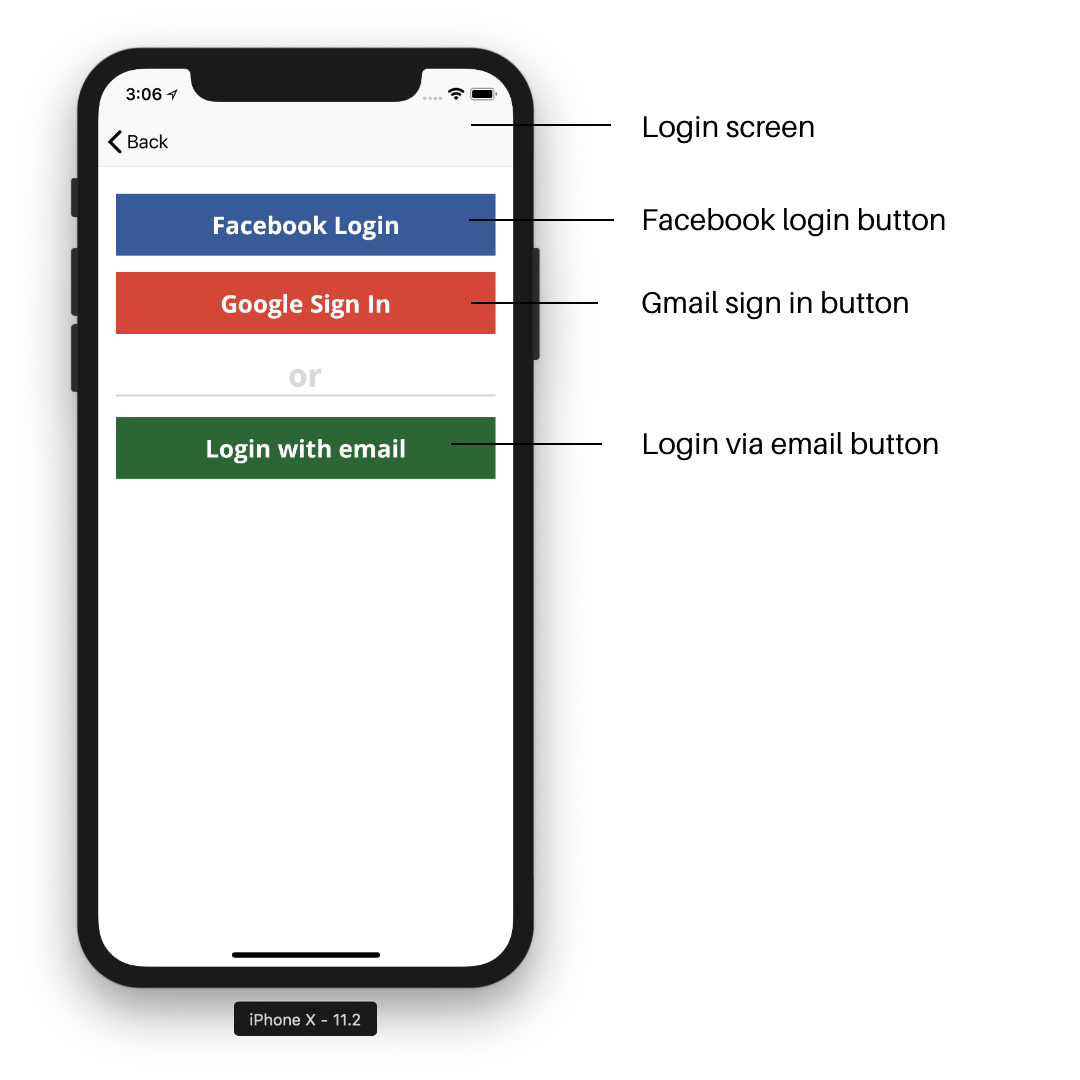
\includegraphics[width=0.50\linewidth]{figures/ch2/loginOptions.png}
            \caption{\label{fig:loginOptions} Login options in the app}
    \end{figure}
    
     \textbf{1. Login via Social Accounts}
     \begin{itemize}
         \item Facebook login
         \item Gmail login
     \end{itemize}
   
     \textbf{2. Login via Email} \\
    This screen requires your credentials to enter the application. The screen has appeared in Figure~\ref{fig:login_email}.
     
     \begin{figure}[H]
            \centering
            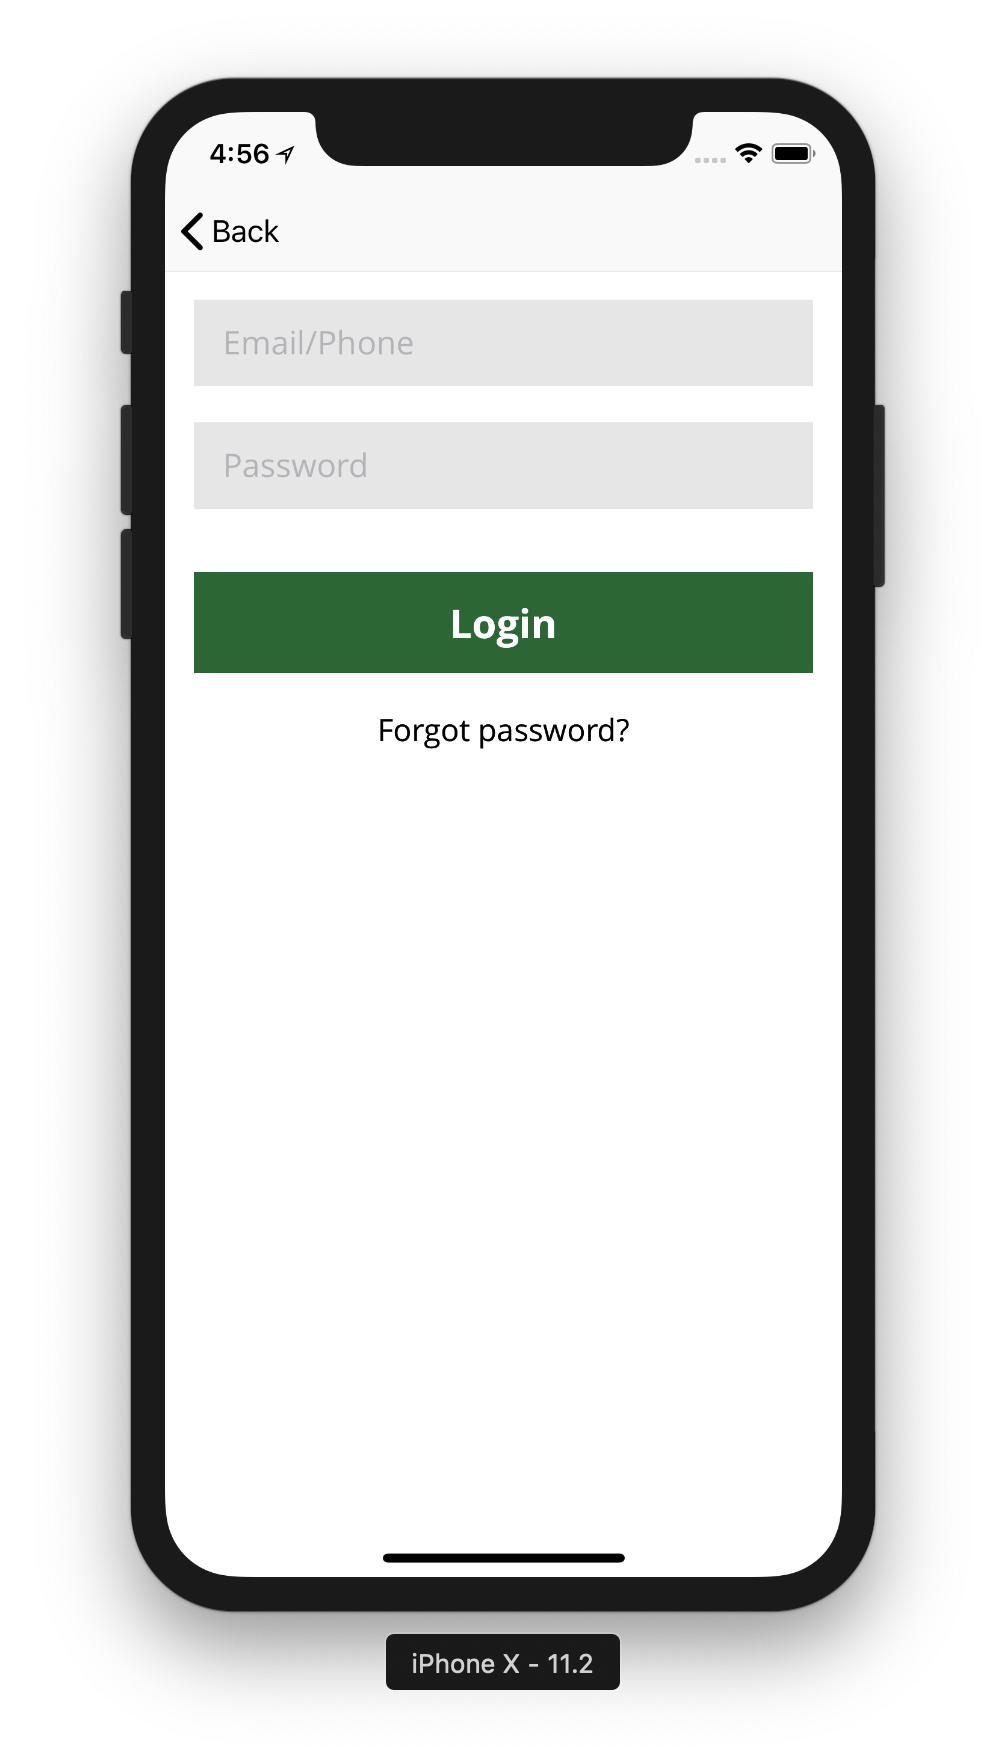
\includegraphics[width=0.50\linewidth]{figures/ch2/login_email.png}
            \caption{\label{fig:login_email} Login via email}
    \end{figure}
    
    
    \item \textbf{Home} \\
    When you log in in the application, straight way, you arrive on the home screen which fundamentally has everything what you need to use the application.
    
    \begin{figure}[H]
            \centering
            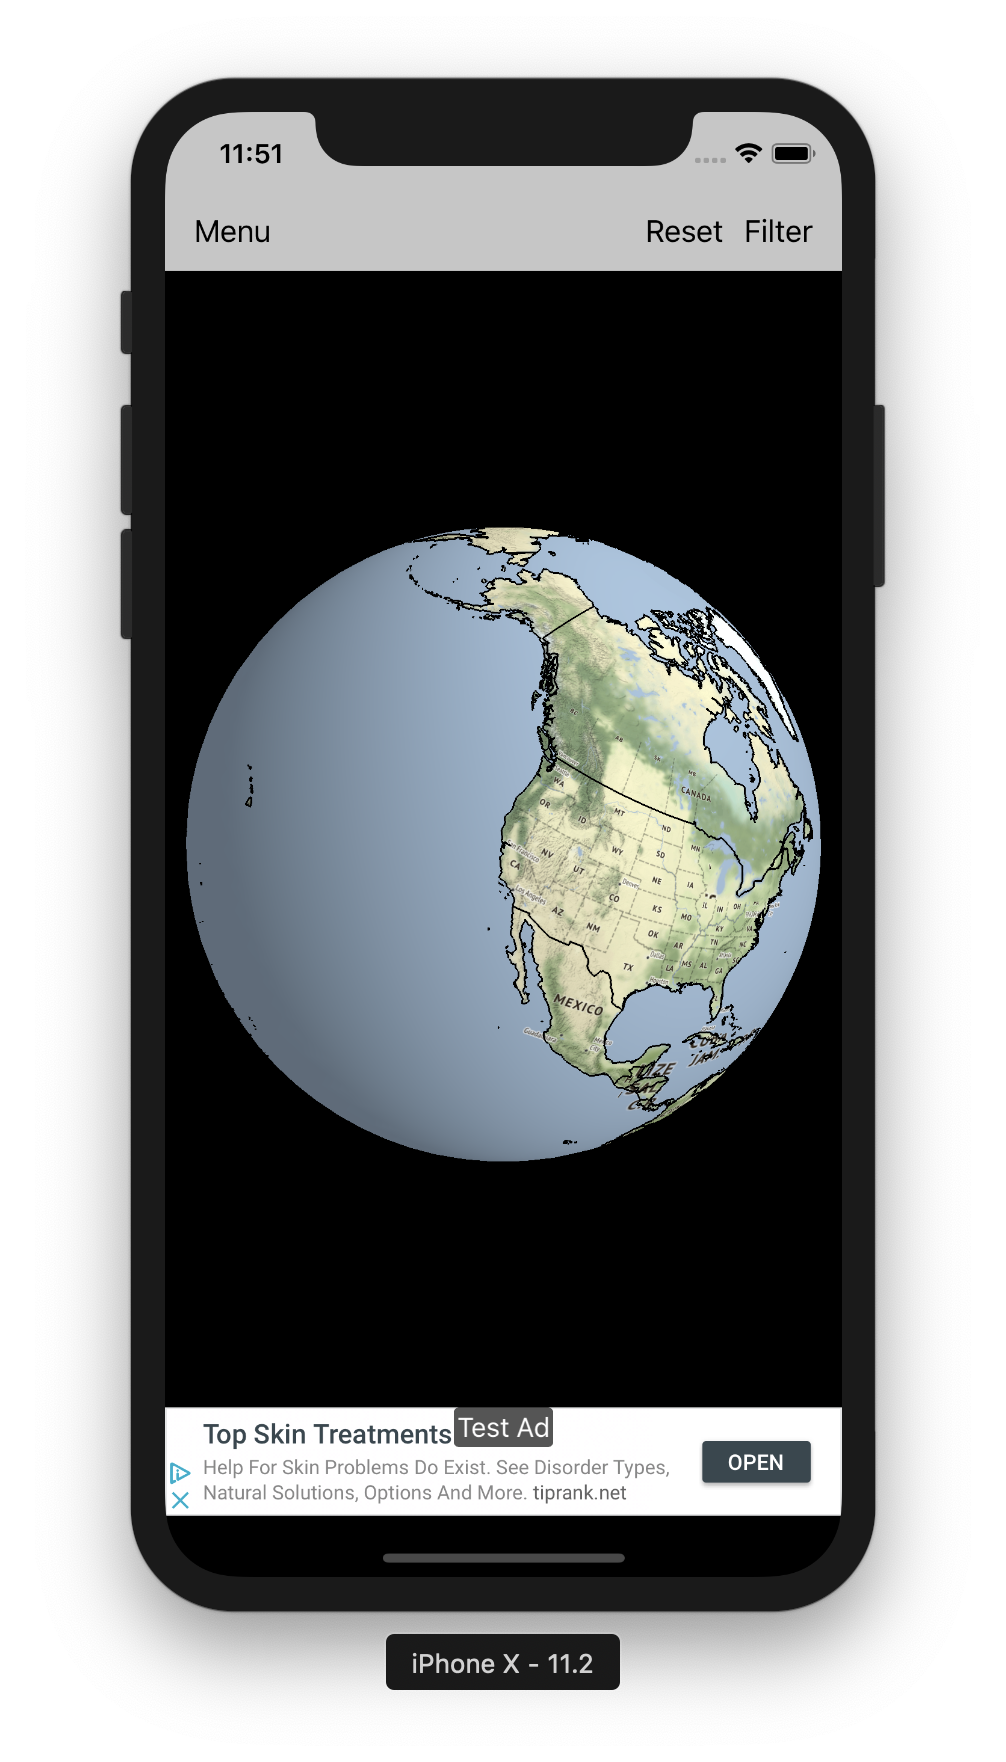
\includegraphics[width=0.5\linewidth]{figures/ch2/home.png}
            \caption{\label{fig:home_screen} Home page - landing page after login}
    \end{figure}
    

    \item \textbf{Slide out menu} \\
    Slide out menu has been utilized to give the application an extremely pleasant look in light of keeping the ease of use while exploring in the application. It has been shown in Figure~\ref{fig:side_menu}.
    
     \begin{figure}[H]
            \centering
            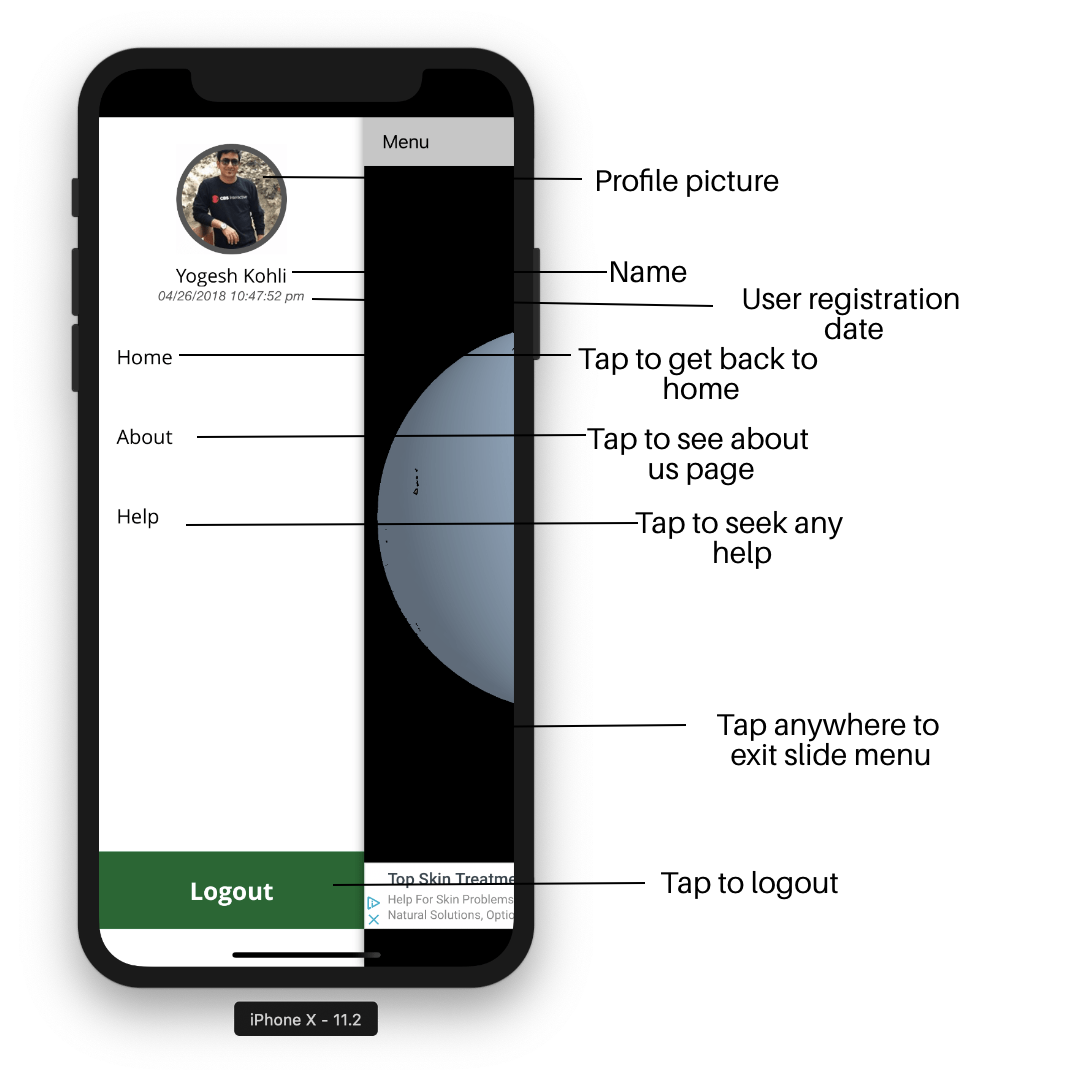
\includegraphics[width=0.50\linewidth]{figures/ch2/side_menu.png}
            \caption{\label{fig:side_menu} Slide out menu after selecting menu option on Home screen}
    \end{figure}
    
    
   \item \textbf{Filter screens} \\
    Tapping on filter button on home screen takes you to Figure~\ref{fig:filter_screen}.
    
    \begin{figure}[H]
            \centering
            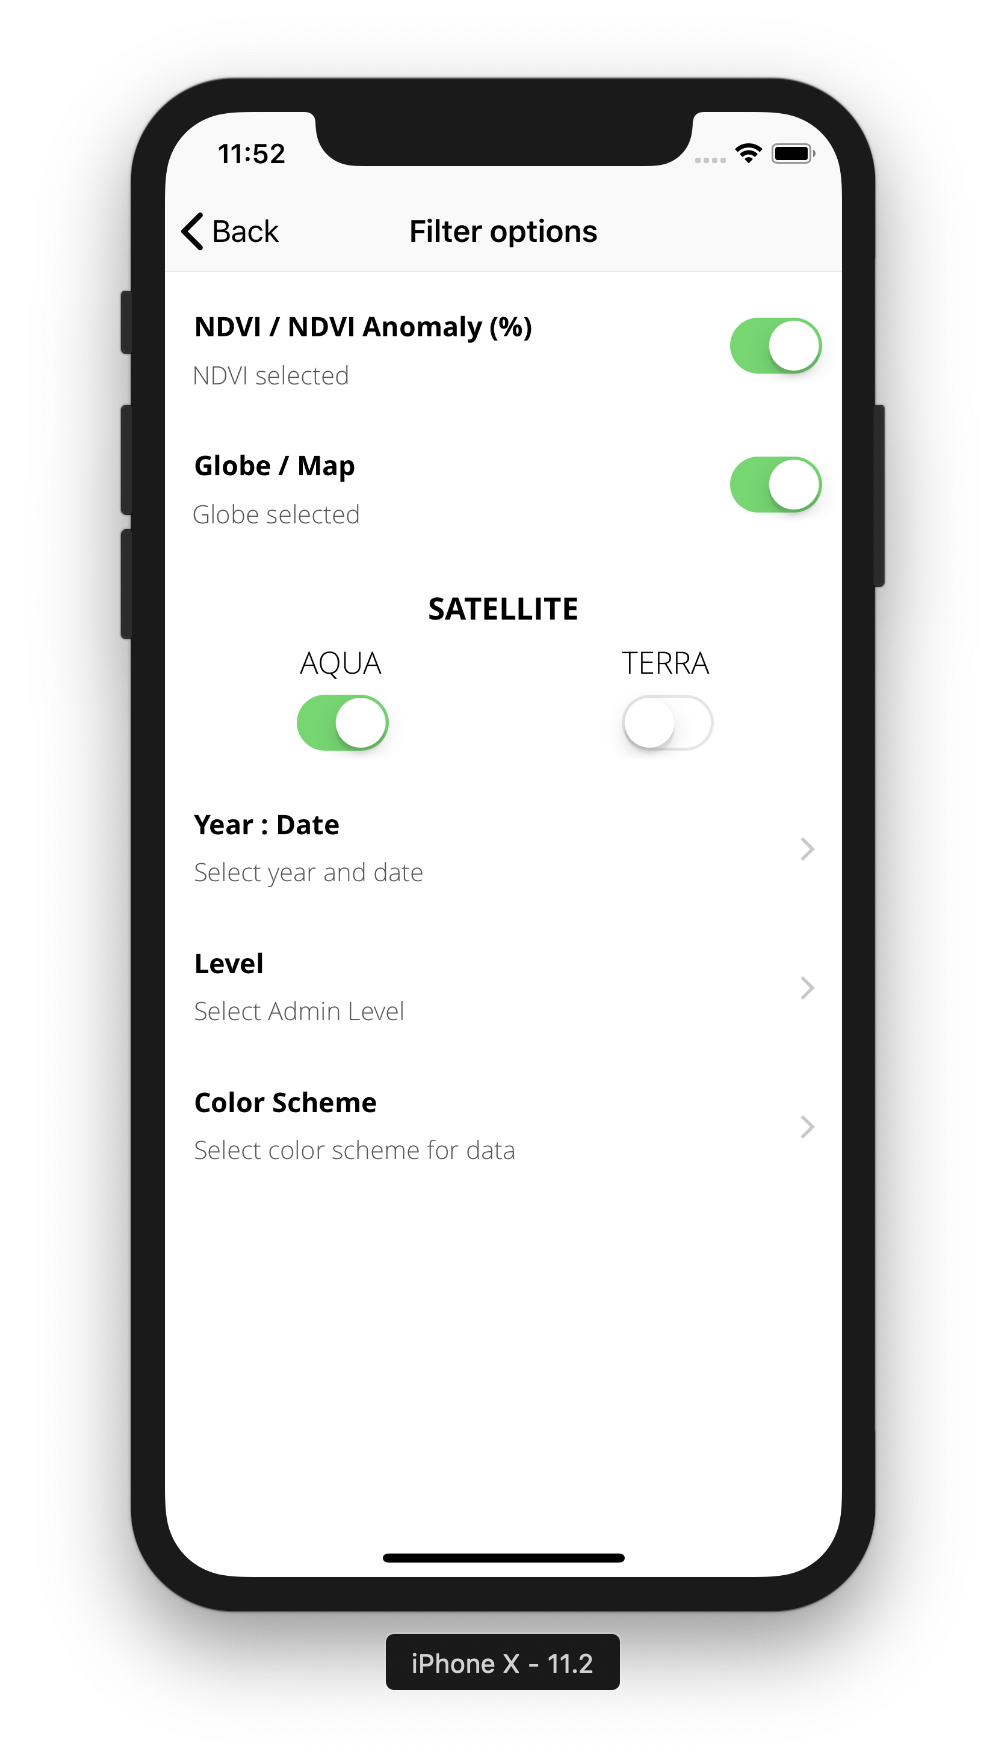
\includegraphics[width=0.50\linewidth]{figures/ch2/filter_screen.png}
            \caption{\label{fig:filter_screen} Filter screen after selecting filter option on Home screen}
    \end{figure}
    
    Now, you have various ways to filter your data.
   
    \begin{itemize}
        \item \textbf{Year list}
        
        Year - Date wise tap on filter screen takes you here, shown in Figure~\ref{fig:years_list_screen}.
        
         \begin{figure}[H]
            \centering
            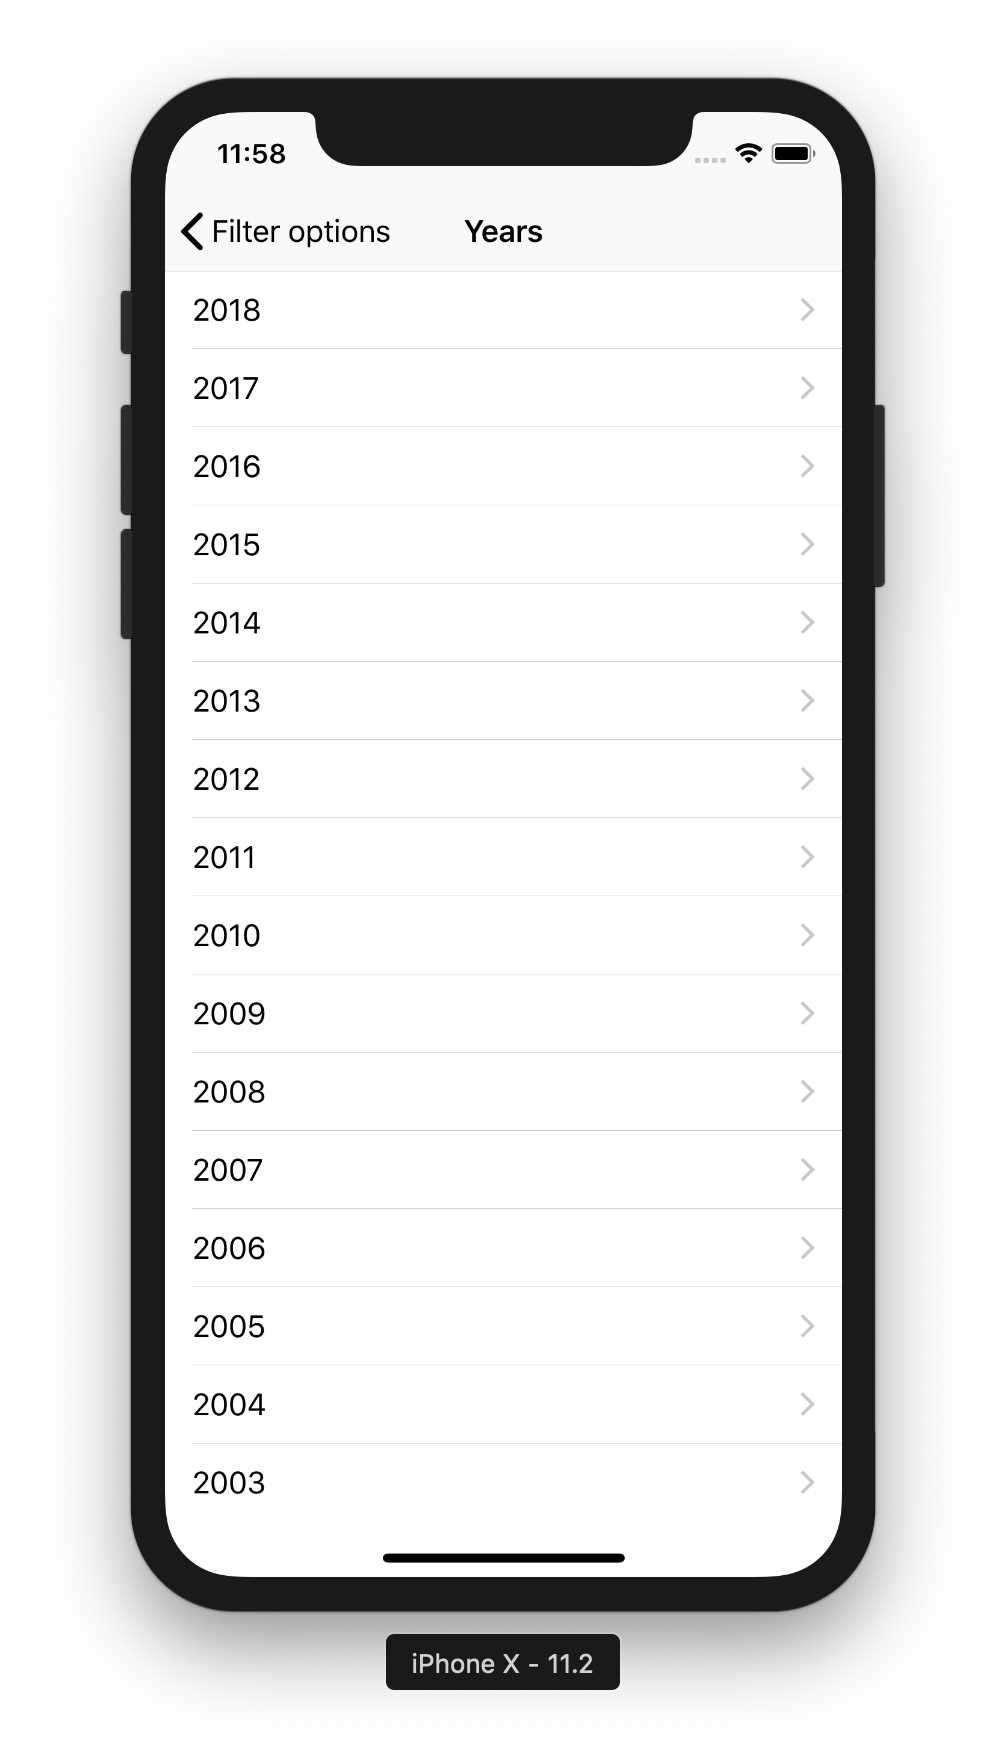
\includegraphics[width=0.50\linewidth]{figures/ch2/year_list.png}
            \caption{\label{fig:years_list_screen} Filter - Year list screen}
    \end{figure}
   
        \item \textbf{Admin level list}
        
        Admin Level tap takes you here, shown in Figure~\ref{fig:level_list_screen}.
        
         \begin{figure}[H]
            \centering
            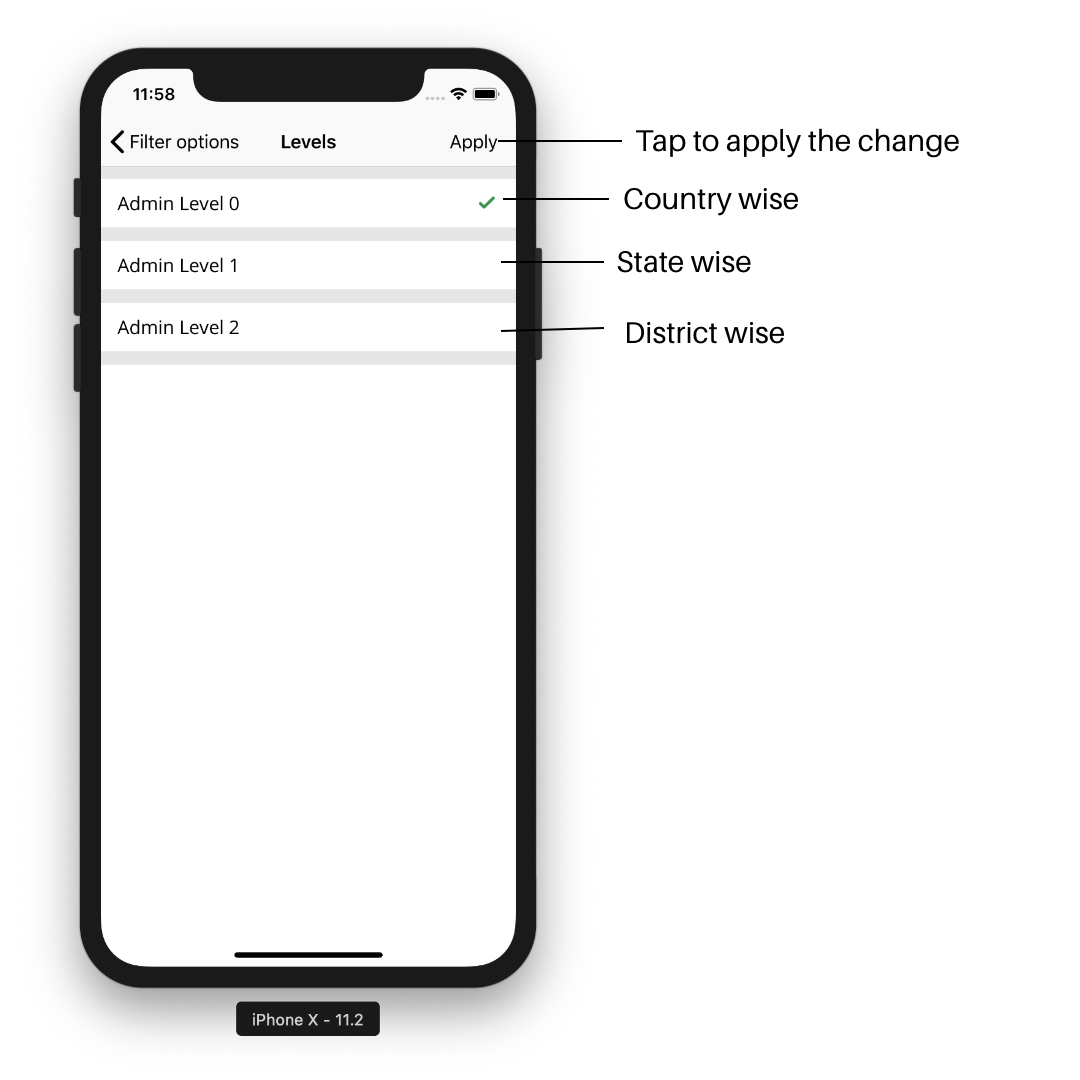
\includegraphics[width=0.50\linewidth]{figures/ch2/level_list.png}
            \caption{\label{fig:level_list_screen} Filter - Admin level list screen}
        \end{figure}

     \item \textbf{Color scheme list}
     
     Color scheme tap takes you here, shown in Figure~\ref{fig:color_scheme}.
        
        \begin{figure}[H]
            \centering
            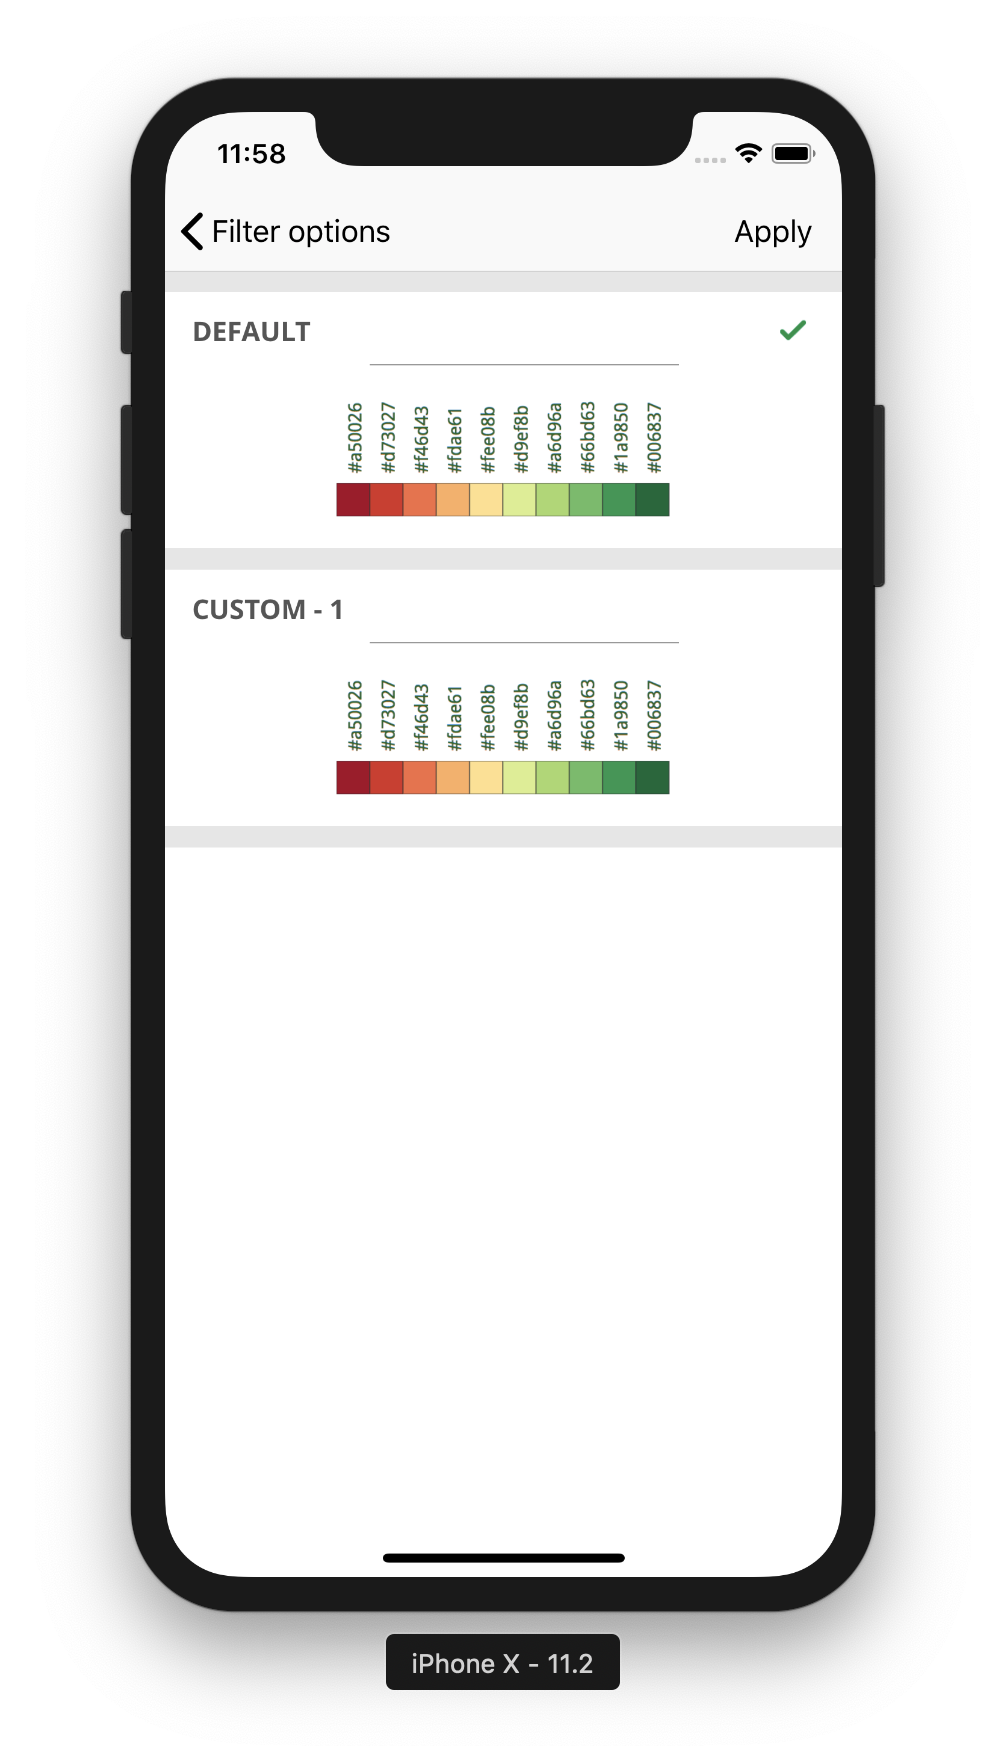
\includegraphics[width=0.50\linewidth]{figures/ch2/color_scheme.png}
            \caption{\label{fig:color_scheme} Filter - Color palette  options screen}
        \end{figure}
        
    \end{itemize}

\end{itemize}



